\chapter{To verify truth table of XNOR gate}

\section{Apparatus}
%\label{sec:objectives}
	\begin{itemize}
		\tightlist
		\item Kit for realization of gates
		\item Connecting Leads
	\end{itemize}

\section{Theory}
	The 'Exclusive-NOR' gate circuit does the opposite to the EX-OR gate. It will give a low output if either, but not both of its two inputs are high. The symbol is an EX-OR gate with a small circle on the output. The small circle represents inversion.
	\begin{figure}[h]
		\centering
		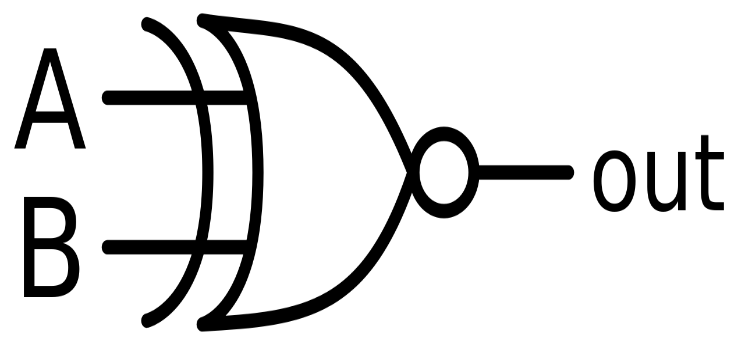
\includegraphics{img/exp7/1}
		\caption{Symbol for XNOR gate}
		\label{fig:7:1}
	\end{figure}
	\begin{figure}[h]
		\centering
		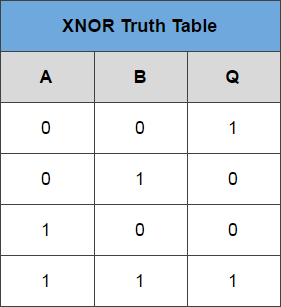
\includegraphics{img/exp7/2}
		\caption{Truth Table for XNOR gate}
		\label{fig:7:2}
	\end{figure}
	
	Ex-NOR gate is created from AND, NOT and OR gates.The output is high only when both the inputs are same.
	
	\begin{figure}[h]
		\centering
		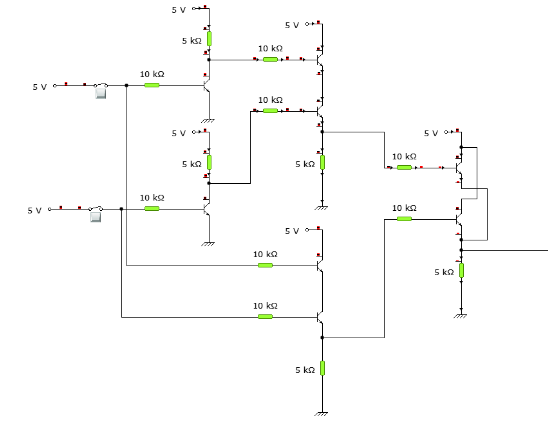
\includegraphics{img/exp7/3}
		\caption{Circut for making XNOR gate}
		\label{fig:7:3}
	\end{figure}
				
\section{Procedure}
	\subsubsection{Simulator 1}
	\begin{itemize}
		\tightlist
		\item Connect the supply(+5V) to the circuit.
		\item Press the switches for inputs "A" and "B".
		\item The bulb glows if both the switches are ON or if both the switches are OFF else it won't glow.
		\item Repeat step-2 and step-3 for all state of inputs.
	\end{itemize}

	\subsubsection{Simulator 2}
	\begin{itemize}
		\tightlist
		\item Enter the Boolean input "A" and "B".
		\item Enter the Boolean output for your corresponding inputs.
		\item Click on "Check" Button to verify your output.
		\item Click "Print" if you want to get print out of Truth Table.
	\end{itemize}


\section{Observations}
	\begin{figure}[h]
		\centering
		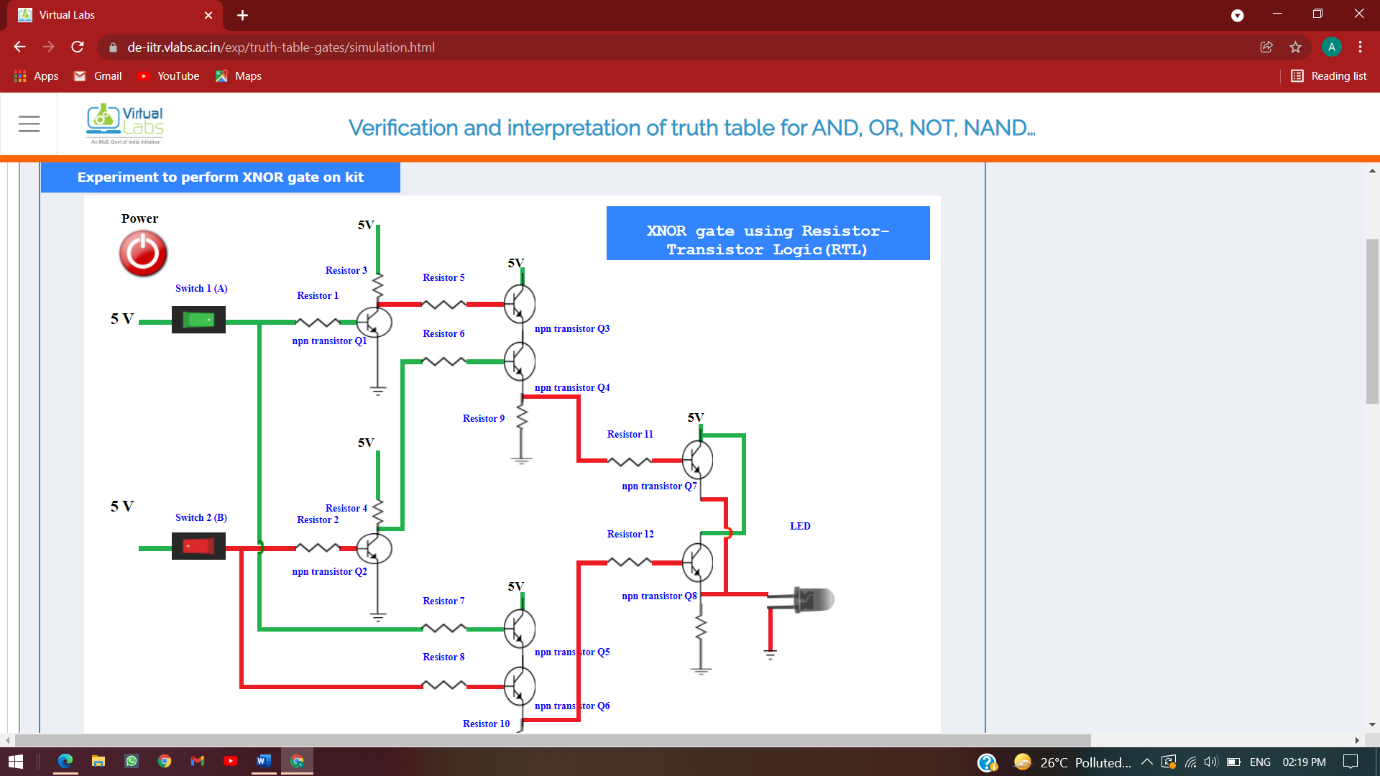
\includegraphics[width=0.9\linewidth]{img/exp7/4}
		\caption{}
		\label{fig:7:4}
	\end{figure}
		\begin{figure}[h]
		\centering
		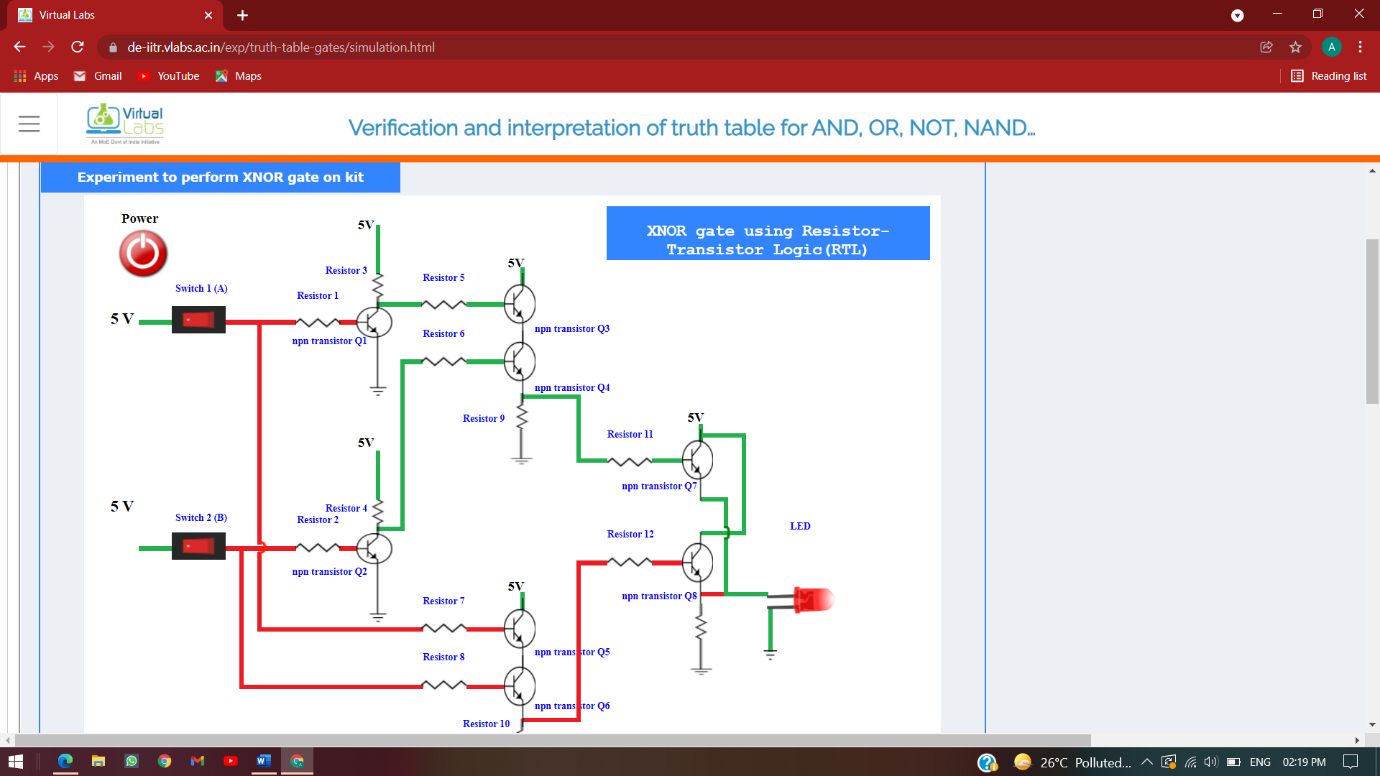
\includegraphics[width=0.9\linewidth]{img/exp7/5}
		\caption{}
		\label{fig:7:5}
	\end{figure}
		\begin{figure}[h]
		\centering
		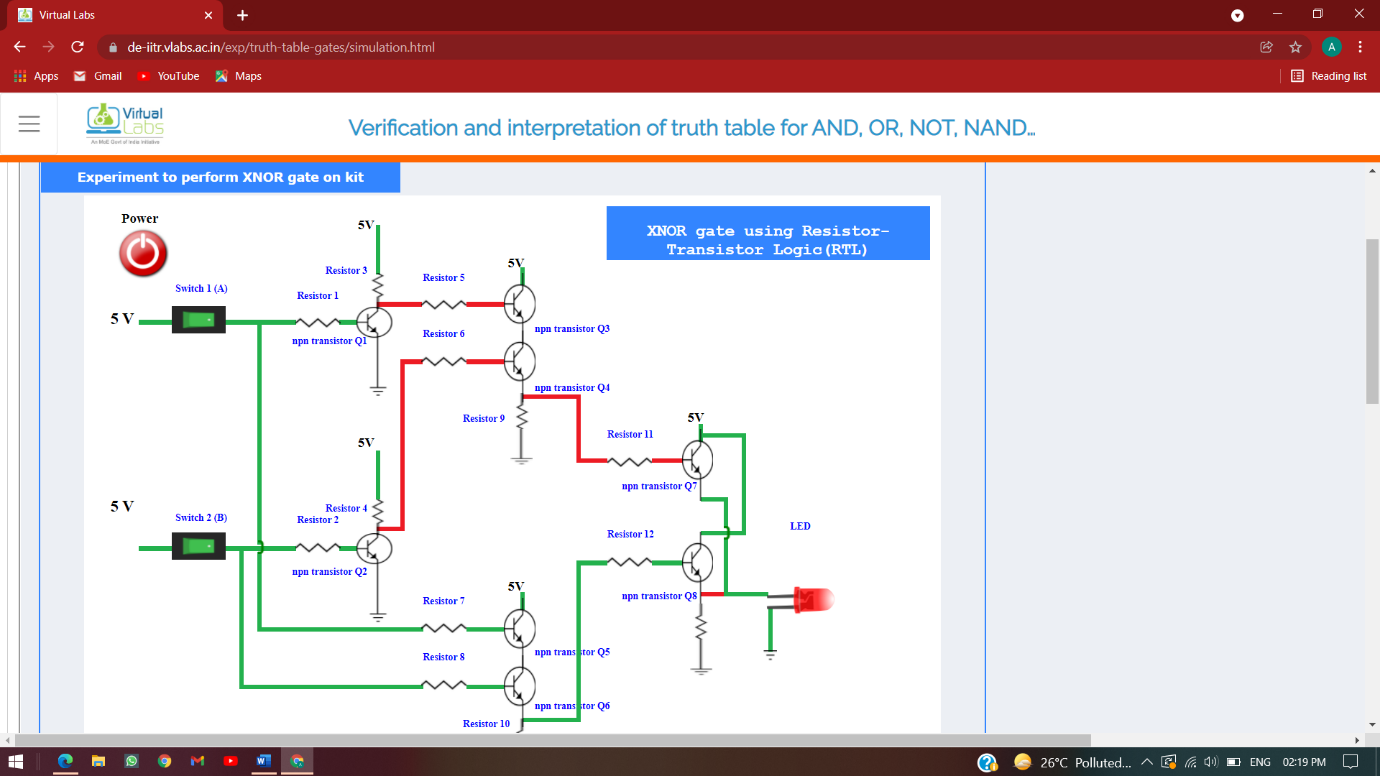
\includegraphics[width=0.9\linewidth]{img/exp7/6}
		\caption{}
		\label{fig:7:6}
	\end{figure}
		\begin{figure}[h]
		\centering
		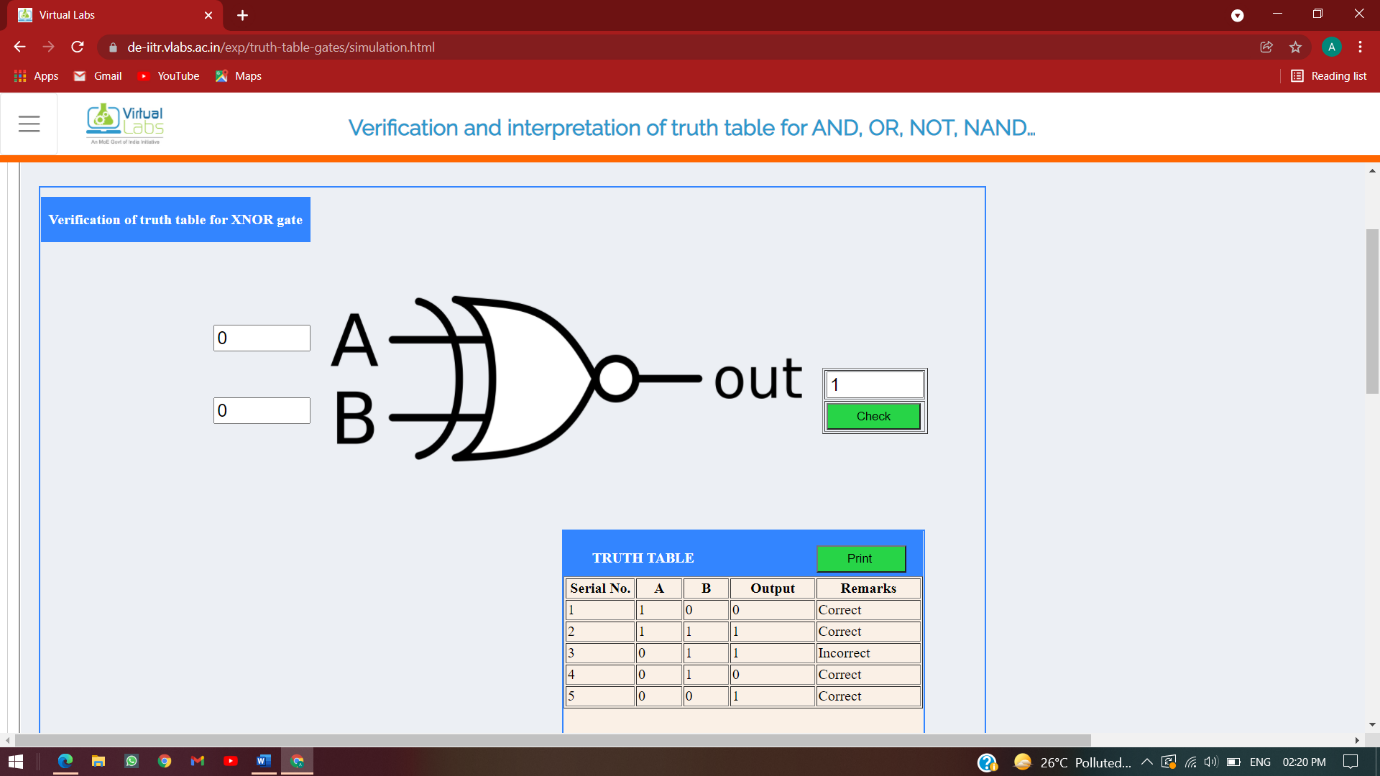
\includegraphics[width=0.9\linewidth]{img/exp7/7}
		\caption{}
		\label{fig:7:7}
	\end{figure}

\section{Conclusion}
XNOR gate basically negates the XOR gate. It gives high output only when both the inputs are same else it gives low output.

\section{Precautions}
	\begin{enumerate}
		\tightlist
		\item Make the connections when power supply is OFF.
		\item Ensure that the connections are tight.
		\item Change the status of inputs only when power supply is OFF.
	\end{enumerate}